\begin{problem}
\begin{staffnotes}
F98 Basic probability, F01.ps10.prob1
\end{staffnotes}

Compute the probabilities of the following three events.\iffalse and
determine which one is most likely.\fi Assume that the dice are fair,
6-sided, and mutually independent.

\begin{problemparts}
\problempart Rolling at least one 6 when six dice are rolled.

\begin{solution}
The probability of rolling a 6 on a particular die is $1/6$.  The
probability of not rolling a 6 on a particular die is $5/6$, since
this is the complementary event.  The probability of not rolling a 6
on any of six dice is $(5/6)^6$, since the numbers rolled are mutually
independent.  The probability of rolling a 6 on some die is therefore
\[
1 - (\frac{5}{6})^6 = 0.665\ldots.
\]
\end{solution}

\problempart Rolling at least two 6's when twelve dice are rolled.

\begin{solution}
The probability of rolling two or more 6's is 1 minus the probability
of rolling zero or one 6's.  The probability of rolling zero 6's is
$(5/6)^{12}$, arguing as before.  The probablity of rolling exactly
one 6 is
\[
12 \cdot \frac{1}{6} \cdot \left(\frac{5}{6}\right)^{11}
\]
since there are 12 ways to choose the die that comes up 6, the
probability of this die coming up 6 is $\cfrac{1}{6}$, and the
probability of the remaining dice all coming up in the range 1 to 5 is
$(5/6)^{11}$.  Overall, the probability of rolling two or more sixes
is therefore
\begin{eqnarray*}
1 - \left(\frac{5}{6}\right)^{12} -
        12 \cdot \frac{1}{6} \cdot \left(\frac{5}{6}\right)^{11}
                & = &   0.618\ldots.
\end{eqnarray*}

\end{solution}

\problempart Rolling at least three 6's when eighteen dice are rolled.

\begin{solution}
Arguing as before, the probability of rolling at least three 6's is


\begin{eqnarray*}
       - \left(\frac{5}{6}\right)^{18}
        - 18 \cdot \frac{1}{6} \cdot \left(\frac{5}{6}\right)^{17}
        - \binom{18}{2} \cdot \left(\frac{1}{6}\right)^2 \cdot
                \left(\frac{5}{6}\right)^{16}
        & = &   0.597\ldots.
\end{eqnarray*}
\end{solution}

\end{problemparts}

\begin{solution}
The first event is most likely.
\end{solution}
\end{problem}


\begin{problem}
\begin{staffnotes}
F00 tournament probabilities, F01.ps10,prob3
\end{staffnotes}

A tennis tournament has eight players, including twins Al and Bert.
The players are assigned randomly to positions in the first round of a
tournament ladder (see Figure~\ref{tennis}).

\begin{figure}%[htbp]
%\centerline{\psfig{figure=/a/class/6.042/fall00/handouts/fig/H64-tennis.eps,height=4in}}
\centerline{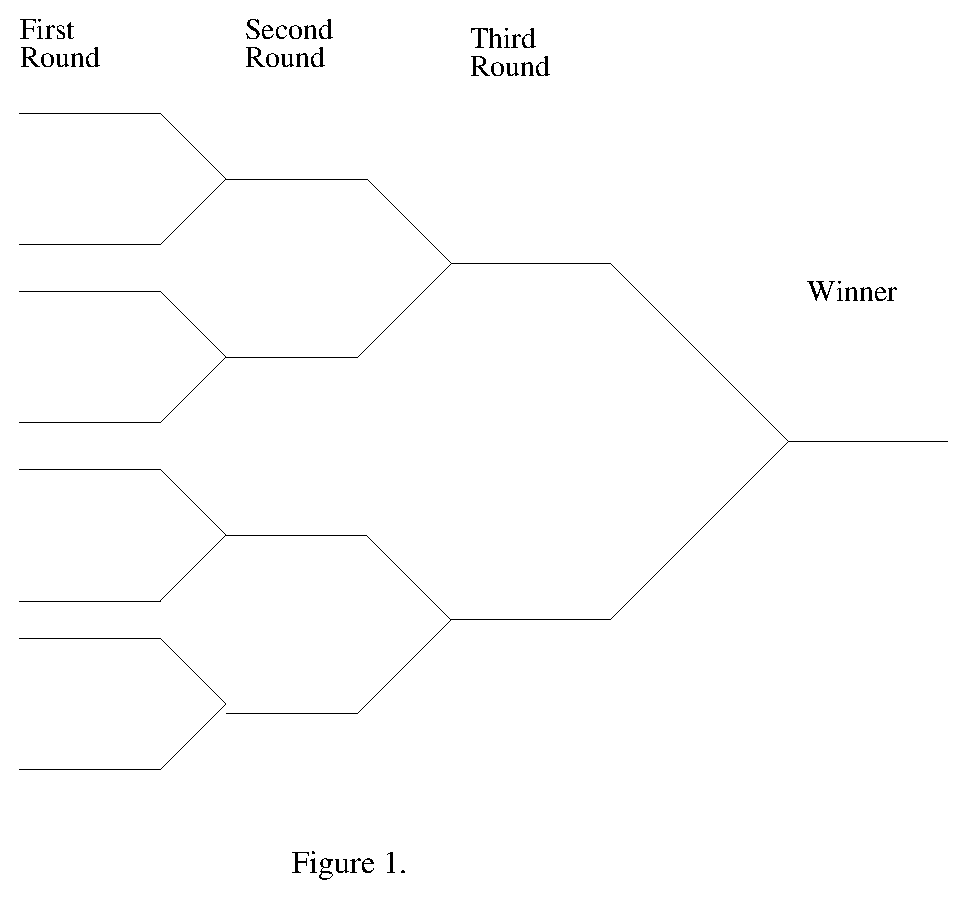
\includegraphics[height=4in]{H64-tennis}}
\caption{Tournament Tree}
\label{tennis}
\end{figure}

\bparts

\ppart
Suppose the best player always defeats everybody else, and
the second-best player always defeats everybody but the best. What
is the chance that the second-best player makes it to the final round?

\begin{solution}
In order to make it to the final round, the
second-best player has to meet
the winner in the final round and not earlier.
That happens if and only if the best
player and the second-best player start out in different brackets of
four; in other words, if the best player starts in position 1-4 of the
first round, then the second-best must start in positions 5-8, and
vice versa.

Here are two ways to determine the probability.  The first way counts
complete assignments: there are 8 ways to place the best player in the
first round, then 4 ways to place the second-best, then $6!$ ways to
place the remaining players.  Divide by the size of the sample space
($8!$, the total number of ways to assign all eight players with no
constraints) to get $4/7$.

The second way treats the second player's position as a random selection.
The best player can be placed anywhere.  Given the best player's position,
the second-best player will meet the first player in the final round
only if he is placed in 4 of the remaining 7 positions---not 4 out of 8,
because the best player is already occupying one (this is a common error
-- the positions of the players can't be treated like independent coin
flips or dice rolls, because no two players can occupy the same
position.)!  Since all placements are equally likely, there is a $4/7$
chance of this happening.
\end{solution}

\ppart Suppose the eight tennis players are equally good, that is, for
any match between two players $A$ and $B$,
\[
\prob{A \mbox{ wins}}=\prob{B \mbox{ wins}}= 1/2,
\]

What is the chance that the twins Al and Bert ever meet in a match
during the tournament?

\begin{solution}

The probability that Al and Bert will meet in the first round is $1/7$
(Al can be placed anywhere, but given Al's position, Bert has only 1
choice in 7).

Al and Bert will meet in the second round if and only if both win
their first-round matches (with probability $1/2 \cdot 1/2$) and both
are in different groups of two but the same group of four (probability
$2/7$).

They will meet in the third round if and only if both win two matches
(with probability $1/2^2 \cdot 1/2^2$) and both are in different
groups of four (probability $4/7$).

Since these events are disjoint, the probability that they meet in any
round is just the sum:
\[
\frac{1}{7} + \frac{1}{2} \cdot \frac{1}{2} \cdot \frac{2}{7}
+ \frac{1}{4} \cdot \frac{1}{4} \cdot \frac{4}{7} = \frac{1}{4}
\]
\end{solution}

\eparts

\end{problem}


\begin{problem}
\begin{staffnotes}
\TBA{NEEDS SOLUTION}
\end{staffnotes}

Let us look at a variant of the Monty Hall problem.  We have three
contestants: Alice, Bob, and Charlie, and each one is given an apple.
Two of the apples contain worms, and the third is a really great Red
Delicious.  As soon as the game starts, Monty Hall tells one of the
contestants with a worm (say, Bob) to bite into their apple.  Bob then
sees the worm and leaves.  Alice and Charlie then have to decide
whether they want to keep their own apple, or to switch apples with
the other contestant.

To both Alice and Charlie, the problem looks almost exactly like the
original Monty Hall problem.  Each of them has just seen one of the
"bad prizes" revealed, and they now know that one of the two remaining
prizes is the good one.  If they use the same logic from the original
problem, then they should both want to switch!  Does this make sense,
or is has something changed in this problem?

\bparts

\ppart Use the four step method to determine the probability that
Alice will win if she keeps her apple.

\begin{solution}
\TBA{To be added}
\end{solution}

\ppart Now, determine the probability that Alice will win if she
switches apples with Charlie.  Should she switch?

\begin{solution}
\TBA{To be added}
\end{solution}

\ppart Is this the same result that was obtained for the original
Monty Hall problem?  If it is different, explain how this problem
differs from the original Monty Hall problem and why this should
provide a different result.

\begin{solution}
\TBA{To be added}
\end{solution}

\eparts

\end{problem}

\begin{problem} 
\begin{staffnotes}
\textbf{S17 Dylan: Quantifiers}:
\end{staffnotes}

Consider the following predicates where the universe of discourse is
the set of all living things:
\begin{description}
\item[$P(x)$:] $x$ is a monkey
\item[$Q(x)$:] $x$ is a 6.042 TA
\item[$R(x)$:] $x$ comes from the 23rd century
\item[$S(x)$:] $x$ likes to eat pizza
\end{description}
Express each of the following statements using quantifiers, logical
connectives, and/or the above predicates.

\begin{problemparts}
\ppart No monkeys like to eat pizza.

\begin{solution}
$\forall x.\ P(x) \QIMPLIES \QNOT(S(x))$
\end{solution}

\ppart Nobody from the 23rd century dislikes eating pizza.

\begin{solution}
$\forall x.\ R(x) \QIMPLIES S(x)$
\end{solution}

\ppart All 6.042 TAs are monkeys.

\begin{solution}
$\forall x.\ Q(x) \QIMPLIES P(x)$
\end{solution}

\ppart  No 6.042 TA comes from the 23rd century.

\begin{solution}
$\forall x.\ Q(x) \QIMPLIES \QNOT(R(x))$
\end{solution}

\ppart Does (d) follow logically from (a), (b), and (c)?  If so, give
a proof.  If not, give a counterexample.

\begin{solution}
\begin{center}
\begin{align*}
Q(x) & \QIMPLIES P(x) & \text{(from (c))} \\
P(x) & \QIMPLIES \QNOT S(x) & \text{(from (a))} \\
\QNOT(S(x)) \QIMPLIES \QNOT(R(x)) & \text{(from contrapositive of (b))}\\ 
\therefore Q(x) \QIMPLIES \QNOT R(x)
\end{align*}
\end{center}
\end{solution}

\ppart Translate into English: $\forall x.\, (R(x) \QAND S(x)) \QIMPLIES
Q(x)$.

\begin{solution}
Anyone who is from the 23rd century or  likes to eat pizza is a 6.042 TA.
\end{solution}

\ppart Translate into English:
\[
[\exists x.\, R(x) \QAND \QNOT(Q(x))]
\QIMPLIES \forall x.\,(P(x) \QIMPLIES S(x)).
\]

\begin{solution}
If there is a person from the 23rd century who is not a 6.042 TA then all monkeys like to eat pizza
\end{solution}

\begin{solution}
Some students forgot leading quantifiers in the first parts (especially
$\forall x$). On the last part, many students mistakenly said that
the entity mentioned in the first `if' would be a monkey that liked
pizza. Note that this is not the same as the correct statement.
\end{solution}

\end{problemparts}
\end{problem}

\begin{problem}
restore probability parts FP_rogue_pair
\end{problem}

\begin{staffnotes}
tedious, overlong
F07.Ps10.Prob4, F08.ps11.prob4
check for more recent version
\end{staffnotes}

\begin{problem}
Independently flip three fair coins (with ``fair'' meaning ``equally likely to come
up with a head or a tail").
\begin{itemize}
\item Let $H_i$ be the indicator variable for a head occurring on the $i$th flip, for $i=1,2,3$,
\item $C$ be the random variable for the number of heads flipped, $H_1+H_2+H_3$,
\item $M$ to be the indicator variable for the event that all three coins match, $[H_1=H_2=H_3]$,
\item and $S$ be the indicator variable for the event that an odd number of heads are flipped, $[C \equiv 1 \mod 2]$.
\end{itemize}

\bparts

\ppart\label{depC} Show that none of these six variables is independent of $C$.

\hint Consider the case when $C=3$.

\begin{solution}
If $C=3$, then the values of all the other variables are determined, namely $H_1=H_2=H_3=M=S=1$.  

Therefore, for all six variables $V$, $\prcond{V=1}{C=3} = 1$, but $\pr{V=1}\neq 1$. So
\[
\prcond{V=1}{C=3} \neq \pr{V=1}
\]
for all six variables, $V$, which shows that none of them is independent of $C$.
\end{solution}

\ppart Show that $M$ and $S$ are pairwise independent.

\begin{solution}
To see that $M$ and $S$ are pairwise independent, we check each of the cases.
\begin{align*}
\pr{S=0 \text{ and } M=0} & = \pr{HHT,HTH,THH}\\
    & = \frac{3}{8} = \frac{1}{2} \cdot \frac{3}{4} =\pr{S=0} \cdot \pr{M = 0}\\
\pr{S=0 \text{ and } M=1} & = \pr{TTT}\\
    & = \frac{1}{8} = \frac{1}{2} \cdot \frac{1}{4} =\pr{S=0} \cdot \pr{M = 1}\\
\pr{S=1 \text{ and } M=0} & = \pr{TTH,THT,HTT}\\
    & = \frac{3}{8} = \frac{1}{2} \cdot \frac{3}{4} =\pr{S = 1} \cdot \pr{M = 0}\\
\pr{S=1 \text{ and } M=1} & = \pr{HHH}\\
    & = \frac{1}{8} = \frac{1}{2} \cdot \frac{1}{4} =\pr{S = 1} \cdot \pr{M = 1}.
\end{align*}
\end{solution}

\ppart\label{H123S} Show that $H_1,H_2,H_3$, and $S$ are 3-wise
independent, but not mutually independent.

\begin{solution}
Since $H_1,H_2,H_3$ determine all the other variables, then by
the same kind of argument used in part~\eqref{depC}, no set of four or
more variables including these three can be mutually independent.

The variables $H_1,H_2,H_3$ are 3-wise independent by definition of
``flipping independently.''  Now consider the three variables $H_1,H_2,S$.
\begin{align*}
\lefteqn{\pr{S=a \text{ and } H_1=b \text{ and } H_2=c}}\\
  & = \pr{(b+c+H_3 \equiv a \mod 2) \text{ and } H_1=b \text{ and } H_2=c}
      & ([S=a] ::= [H_1+H_2+H_3 \equiv a \mod 2])\\
  & = \pr{H_3 = rem(a-b-c,2) \text{ and } H_1=b \text{ and }
  H_2=c}\\
  & = \pr{H_3 = rem(a-b-c,2)}\cdot \pr{H_1=b} \cdot \pr{H_2=c} &
  \text{(independence of the flips)} \\
& = (1/2)^3 \\
& = \pr{S=a} \cdot \pr{H_1=b} \cdot \pr{H_2=c} &
  \text{(since $\pr{S=a}=1/2$)}.
\end{align*}
Likewise for $S$ and any other two $H_i$'s.  So $H_1,H_2,H_3$, and $S$ are
3-wise independent because any three of them are mutually independent.
\end{solution}

\iffalse
\ppart Show that the five variables other than $C$ are pairwise independent.

\begin{solution}

Part~\eqref{H123S} already shows that any two of $H_1,H_2,H_3,$ and $S$
are pairwise independent, so we need only verify that $H_i$ and $M$ are
pairwise independent and that $S$ and $M$ are pairwise independent.

To see that $H_i$ and $M$ are pairwise independent, we just check the cases where $i = 1$ and $H_1 =1$. The other cases are symmetric.
\begin{align*}
\pr{H_1=1 \text{ and } M=0} & = \pr{HTT, HHT, HTH}\\
    & = \frac{3}{8} = \frac{1}{2} \cdot \frac{3}{4} =\pr{H_1 = 1} \cdot \pr{M = 0}\\
\pr{H_1=1 \text{ and } M=1} & = \pr{HHH}\\
    & = \frac{1}{8} = \frac{1}{2} \cdot \frac{1}{4} =\pr{H_1 = 1} \cdot \pr{M = 1}.
\end{align*}

To see that $S$ and $M$ are pairwise independent, we check each of the cases.
\begin{align*}
\pr{S=0 \text{ and } M=0} & = \pr{HHT,HTH,THH}\\
    & = \frac{3}{8} = \frac{1}{2} \cdot \frac{3}{4} =\pr{S=0} \cdot \pr{M = 0}\\
\pr{S=0 \text{ and } M=1} & = \pr{TTT}\\
    & = \frac{1}{8} = \frac{1}{2} \cdot \frac{1}{4} =\pr{S=0} \cdot \pr{M = 1}\\
\pr{S=1 \text{ and } M=0} & = \pr{TTH,THT,HTT}\\
    & = \frac{3}{8} = \frac{1}{2} \cdot \frac{3}{4} =\pr{S = 1} \cdot \pr{M = 0}\\
\pr{S=1 \text{ and } M=1} & = \pr{HHH}\\
    & = \frac{1}{8} = \frac{1}{2} \cdot \frac{1}{4} =\pr{S = 1} \cdot \pr{M = 1}.
\end{align*}

\end{solution}

\ppart Show that $H_1,S$ and $M$  are not mutually independent.

\begin{solution}
If $H_1=1$ and $S=0$, then $M=0$.  Hence,

\begin{align*}
\pr{H_1=1 \text{ and } S=0 \text{ and } M=0} & = \pr{H_1=1 \text{ and } S=0}\\
    & = \pr{H_1=1}\cdot \pr{S=0}  & \text{(part~\eqref{H123S})}\\
    & = \frac{1}{2} \cdot  \frac{1}{2}\\
    & \textcolor{red}{\neq} \frac{1}{2} \cdot  \frac{1}{2} \cdot \frac{3}{4}\\
    & = \pr{H_1=1}\cdot \pr{S=0} \cdot \pr{M=0}.
\end{align*}
\end{solution}

\ppart Show that no set of three variables including both $M$ and $H_i$
for any $i\in \set{1,2,3}$ is 3-wise independent.

\begin{solution}

We've seen that $H_1,S$, and $M$ are not mutually independent.
  The same reasoning can be applied when substituting $H_2$ or $H_3$ for
  $H_1$.  We've also seen that none of the variables is independent of
  $C$, so $C$ cannot be one of the three variables in the set and still
  have the set be 3-wise independent.

  That leaves sets of the form $\set{M, H_i, H_j}$, $i$ and $j$ not equal
  and between 1 and 3.  If $H_i = H_j = M = 1$, then all coins are heads.

\begin{align*}
\pr{H_i=1 \text{ and } H_j = 1 \text{ and } M=1} & = \pr{H_1=1 \text{ and } H_2 = 1 \text{ and } H_3 =1}\\
    & = \pr{H_1=1}\cdot \pr{H_2 = 1} \cdot \pr{H_3 = 1}  & \text{(indep. of $H_i$'s)}\\
    & = \frac{1}{2} \cdot  \frac{1}{2} \cdot \frac{1}{2}\\
    & \textcolor{red}{\neq} \frac{1}{2} \cdot  \frac{1}{2} \cdot \frac{1}{4}\\
    & = \pr{H_i=1}\cdot \pr{H_j=1} \cdot \pr{M=1}.
\end{align*}
\end{solution}
\fi

\eparts
\end{problem}


\begin{problem}   %ad hoc asymptotic approx formulas
In lecture we discussed the Birthday Paradox.  Namely, we found that
in a group of $m$ people with $N$ possible birthdays, if $m \ll N$,
then:
\[
\pr{\text{all $m$ birthdays are different}} \sim e^{-\frac{m(m-1)}{2N}}
\]
To find the number of people, $m$, necessary for a half chance of a
match, we set the probability to $1/2$ to get:
\[
m \sim \sqrt{(2\ln2)N} \approx 1.18\sqrt{N}
\]

For $N = 365$ days we found $m$ to be 23.

We could also run a different experiment. As we put on the board the
birthdays of the people surveyed, we could ask the class if anyone has
the same birthday. In this case, before we reached a match amongst the
surveyed people, we would already have found other people in the rest
of the class who have the same birthday as someone already
surveyed. Let's investigate why this is.

\bparts

\ppart Consider a group of $m$ people with $N$ possible birthdays
amongst a larger class of $k$ people, such that $m \leq k$. Define
$\pr{A}$ to be the probability that $m$ people all have different
birthdays \textit{and} none of the other $k-m$ people have the same
birthday as one of the $m$.

Show that, if $m \ll N$, then $\pr{A} \sim
e^{\frac{m(m-2k)}{2N}}$. (Notice that the probability of no match is
$e^{-\frac{m^2}{2N}}$ when $k$ is $m$, and it gets smaller as $k$ gets
larger.)

\hspace{0.5in} \textit{Hints:} For $m \ll N$: $\frac{N!}{(N-m)!N^m}
\sim e^{-\frac{m^2}{2N}}$, and $(1-\frac{m}{N}) \sim
e^{-\frac{m}{N}}$.

\begin{solution}

We know:
\[
\pr{A} = \frac{N(N-1)\ldots(N-m+1)\cdot(N-m)^{k-m}}{N^k}
\]

since there are $N$ choices for the first birthday, $N-1$ choices for
the second birthday, etc., for the first $m$ birthdays, and $N-m$
choices for each of the remaining $k-m$ birthdays. There are total
$N^k$ possible combinations of birthdays within the class.

\begin{align*}
\pr{A} &= \frac{N(N-1)\ldots(N-m+1)\cdot(N-m)^{k-m}}{N^k} \\
&= \frac{N!}{(N-m)!}\left(\frac{(N-m)^{k-m}}{N^k}\right) \\
&= \frac{N!}{(N-m)!N^m}\left(\frac{N-m}{N}\right)^{k-m} \\
&= \frac{N!}{(N-m)!N^m}\left(1-\frac{m}{N}\right)^{k-m} \\
&\sim e^{-\frac{m^2}{2N}} \cdot e^{-\frac{m}{N}(k-m)} & \text{(by the Hint)} \\
& = e^{\frac{m(m-2k)}{2N}}
\end{align*}
\end{solution}

\ppart Find the approximate number of people in the group, $m$,
necessary for a half chance of a match (your answer will be in the
form of a quadratic). Then simplify your answer to show that, as $k$
gets large (such that $\sqrt{N} \ll k$), then $m \sim
\frac{N\ln2}{k}$.

\hint $x \ll 1$: $\sqrt{1-x} \sim (1-\frac{x}{2})$.

\begin{solution}

Setting $\pr{A} = 1/2$, we get a solution for $m$:

\begin{align*}
1/2 &= e^{\frac{m(m-2k)}{2N}} \\
-2N\ln2 &= m^2 -2km  \\
0 &= m^2-2km + (2N\ln2) \\
m &= \frac{2k \pm \sqrt{(2k)^2 - 4(2N\ln2)}}{2}
\end{align*}

Simplifying the solution under the assumption of large $k$, we find:
\begin{align*}
m &= \frac{2k - \sqrt{4k^2 - 8N\ln2}}{2} & \text{(taking the lower positive root)} \\
&= k - k\sqrt{1 - \frac{2N\ln2}{k^2}} \\
&\sim k  - k \left(1-\frac{2N\ln2}{2k^2}\right) & \text{(by the Hint)} \\
&= \frac{N\ln2}{k}
\end{align*}

\end{solution}

\eparts

\end{problem}


\begin{problem} \textbf{More Counting}
\begin{staffnotes}
 From http://www.maths.lse.ac.uk/Courses/MA311/\#exams

 S01.practicefinal, 2000.final
\end{staffnotes}

A drawer contains six distinguishable pairs of gloves. Six persons,
named A, B, C, D, E, and F, take a left-hand glove and a right-hand
glove (without replacement, so all gloves are gone at the end ).

\bparts

\ppart In how many ways can this selection be done ?

\begin{solution}
$(6!)^2$.
\end{solution}

\ppart In how many ways can this be done such that B has
a non-matching pair and D has a matching pair ?

\begin{solution}
$(6!)(4\cdot4!)$.
\end{solution}

\ppart In how many ways can this be done if exactly four
people have a matching pair ?

\begin{solution}
\[
\binom{6}{4}(6!).
\]
\end{solution}

\ppart In how many ways can this be done such that A
and~B have matching pairs but none of C, D, E, and F have matching
pairs?  \hint For a \emph{particular} choice of left-hand gloves,
consider denoting the set of events in which C gets a matching
right-hand glove by~$M_C$---likewise for all the others.

\begin{solution}
There are $6!$ ways to choose the left-hand gloves.
  Since A and B have matching pairs, we know what they get (no freedom
  there). Now, the remaining 4 must get non-matching pairs. The number
  of choices is equal to the number of derangements of 4 objects (see
  also problem 8d on the practice final), which, by the
  inclusion-exclusion formula, is equal to
  \[
  4!1-\frac{1}{1!}+\frac{1}{2!}-\frac{1}{3!}+\frac{1}{4!}=9
  \]
  therefore, the total number of ways is $6!\cdot 9 = 6480$.
\end{solution}

\iffalse
  \begin{displaymath}
    6!\biggl(
      4!-\binom{4}{1}3!+\binom{4}{2}2!-\binom{4}{3}1!+\binom{4}{4}0!
    \biggr)
    =
    720\cdot15
    =
    10800.
  \end{displaymath}
\fi

\eparts

\end{problem}


\begin{problem} \textbf{Probability Inclusion-Exclusion}
\begin{staffnotes}
From ``A first course in Probability"
p 119, exercise 6
S01 Final
\end{staffnotes}

Prove that if $E_1, E_2,\ldots,E_n$ are mutually independent events, then
\[
\Prob{E_1\union E_2\union \cdots \union E_n} = 1-\prod^n_{i=1}\paren{1-P(E_i)}
\]

\begin{solution}
  \begin{eqnarray*}
    \Pr\left[E_1\union E_2\union \cdots \union E_n\right] &=&
    1 - \Pr\left[\overline{E_1\union E_2\union \cdots \union E_n}\right] \\
    &=&
    1 - \Pr\left[\overline{E_1} \intersect \overline{E_2} \intersect
      \cdots \intersect \overline{E_n}\right] \\
    &=&
    1 - \prod_{i=1}^n\Pr\left[\overline{E_i}\right] \\
    &=&
    1 - \prod_{i=1}^n\bigl(1 - \Pr[E_i]\bigr).
  \end{eqnarray*}
  
  The most common error here was to claim that since the $E_i$ are
  independent, $\Pr(E_1 \union \cdots \union E_n) = \Pr(E_1) + \cdots
  + \Pr(E_n)$. This is false, it holds when the events are disjoint.
\end{solution}

\end{problem}

\begin{problem}
\begin{staffnotes}
S01.pfinal

expectation

kproblem{expectation1}

ksource{Nancy's brain}

ktopics{Expectation, linearity of expectation, expected number of
events that occur, binomial distribution, counting permutations}
\end{staffnotes}

Each of five students in 6.042 independently chooses with equal
probability a random integer from $\set{1,\dots,5}$.

\bparts

\ppart What is the expected number of people who choose the
number that gives their position in alphabetical order?

\begin{solution}
Let $X_i$~be the indicator for the event that the $i$th
  person chooses the correct position, \ie $X_i = 1$ if person~$i$
  chooses the number that gives her\slash his position in alphabetical
  order and $X_i = 0$ otherwise. The number of people choosing the
  correct number is then $X_1 + X_2 + X_3 + X_4 + X_5$, which implies
  that the expected number of people choosing the correct number is
\[
    \sum_{i=1}^5 \expect{X_i} = \sum_{i=1}^5 \prob{X_i = 1}.
\]
  Since every person chooses a number in the range $\set{1,\dots,5}$
  independently with equal probability, $\prob{X_i = 1} = 1/5$.
  Therefore, the expected number of people who choose the number that
  gives their position is~$1$.
\end{solution}

\ppart Give an expression for the probability that
exactly the expected number of people (as given by your answer to
the previous part) choose their correct positions.

\begin{solution}
Let $A$~be the event that exactly one person chooses the
  right position and $A_i$ be the event that (only) person~$i$ chooses
  the right position. Then
\[
    \Pr[A]
    = \Pr[A_1 \union A_2 \union A_3 \union A_4 \union A_5]
    = \sum_{i=1}^5 \Pr[A_i]
\]
  since the~$A_i$ are disjoint. Furthermore,
\[
    \Pr[A_i] = \underbrace{\frac{1}{5}}_{\mathrm{Winner}}
    \underbrace{\biggl(\frac{4}{5}\biggr)^4}_{\mathrm{Losers}}
\]
  for every~$i$, thus $\Pr[A] = (4/5)^4$.
\end{solution}

\eparts

\bigskip

Now suppose the course TA randomly assigns to the five
students \emph{different} numbers in the same range $\set{1,\dots,5}$,
with all assignments equally likely.

\bparts
\ppart Now what is the expected number of people who are
assigned the number that gives their position in alphabetical order?

\begin{solution}
As in part~(a), let $X_i$ be the indicator for the event that
  person~$i$ chooses the number that gives their position in
  alphabetical order and obtain that the expected number of people
  choosing the correct number is
\[
 \sum_{i=1}^5 \expect{X_i} = 5 \prob{X_1  = 1}.
\]
The number of permutations that start with 1 is $4!$, so the
probability that $X_1 = 1$ is $4!/5! = 1/5$.  Therefore, the expected
number of people who choose the number that gives their position in
alphabetical order is $5(1/5) = 1$.
\end{solution}

\ppart Give an expression for the probability that exactly one person
is assigned their correct positions.

\begin{solution}
We need to calculate the number of permutations of five
  elements such that exactly one element is in the right position.
  There are five ways to choose the element that is in the right
  position; we have to multiply this number with the number of ways to
  permute the remaining four elements in such a way that no element is
  in the right position.

  One way to calculate the number of such
  permutations is to use a tree diagram; another is to use
  inclusion-exclusion \`a~la derangements (we did a similar
  problem in Tutorial~11).  To formalize the latter method, let $A$~be
  the set of 4-permutations such that at least one number is in the
  right place. We are interested in the complement of~$A$---the set of
  4-permutations such that no number is in the right place---this set
  contains $4! - |A|$ elements. Now we rewrite $A = A_1 \union A_2 \union
  A_3 \union A_4$, where $A_i$~is the set of permutations that have the
  $i$th element (and possibly also other elements) in the right place
  and use inclusion\slash exclusion:
  \begin{displaymath}
    |A| = \Card{A_1 \union A_2 \union A_3 \union A_4} =
    \sum_i |A_i| - \sum_{i<j} |A_i \intersect A_j|
    + \sum_{i<j<k} |A_i \intersect A_j \intersect A_k| - |A_1 \intersect A_2 \intersect A_3 \intersect A_4|.
  \end{displaymath}
  Now we note that $|A_i| = 3!$ for every~$i$ since we fix the
  position of the $i$th element and can permute the remaining elements
  arbitrarily. Similarly, $|A_i \intersect A_j| = 2!$ and $|A_i \intersect A_j
  \intersect A_k| = 1!$. This gives
\[
|A| = \Card{A_1 \union A_2 \union A_3 \union A_4} =
  \binom{4}{1} \cdot 3! - \binom{4}{2} 2! + \binom{4}{3} 1!
  - \binom{4}{4} 0! = 24 - 12 + 4 - 1 = 15.
\]
  Therefore, the number of permutations of four elements such that no
  number is in the right position is $4! - |A| = 24 - 15 = 9$ and the
  number of permutations of five elements such that exactly one
  element is in the right position is~$45$.  Since the total number of
  permutations is $5! = 120$, the sought probability is $45 / 120 = 3 /
  8$.
\end{solution}

\eparts
\end{problem}


\begin{problem}
\begin{staffnotes}
S01 pfinal IGNORED

expectation

kproblem{expectation2}

ksource{Nancy}

ktopics{Expectation}
\end{staffnotes}

100 students enter a cafeteria with at least 100 very large tables,
one at a time.  As each students enters, he or she looks around to see
if any of his friends are already there.  If so, he/she joins one of
his friends' tables.  If not, he/she starts a new table.

Assume that, for each pair of students, the probability that they are
friends is $p$.  Moreover, all these pair probabilities are
independent.

\bparts

\ppart For the $ith$ person to enter the cafeteria, what is
the probability he/she starts a new table?

\begin{solution}
$(1-p)^{i-1}$
\end{solution}

\ppart What is the expected number of occupied tables after
everyone has entered?

\begin{solution}
Add this from $i = 1$ to $n$.
\end{solution}
\eparts

\end{problem}

\begin{problem}
\begin{staffnotes}
similar already in repo?

S01.pfinal KIGNORED

ksource{David R's Brain}
\end{staffnotes}

There is a casino in St.\ Petersburg where you have the choice of
betting any portion of your wealth on either of two games: in the
first game, you either receive 3 times what you bet or lose it all
with equal probability.  In the second game the casino gives you 1.4
times what you bet with probability 1 (this casino is understandably
very popular).  Each trial of the two games is played simultaneously.

\bparts

\ppart Call $S_1$ and $S_2$ the fraction of your wealth you bet
on the two games (notice $S_1+S_2\leq 1$).  What values of $S_1$ and
$S_2$ maximize the expected value of your wealth after 1 trial?  What
is the maximum expected value of your wealth?
\begin{solution}
$S_1=1$, max is 1.5
\end{solution}

\ppart What strategy maximizes your expected wealth after $n$
trials? 
\begin{solution}
Always have $S_1=1$
\end{solution}

\ppart Using that strategy, what is the probability that after
10 trials, you have more money than you started with? 
\begin{solution}
$1-2^{-10}$
\end{solution}

\examspace
\ppart After $2n$ trials, what is the {\em most likely} number
of trials in game one that are wins.  And what is the probability that
this occurs?

\begin{solution}
$n$, $f_{2n,0.5}(n)\approx $
\end{solution}

\ppart What fraction of your wealth should you bet on each
trial of the two games, if you want to maximize your wealth after $2n$
trials in the most likely case that you found above? (i.e. suppose
that there are that number of wins over the course of the $2n$
trials).  Assume that it is in your interest to have $S_1+S_2=1$.
\begin{solution}
Maximize $(1.4+1.6S_1)^{0.5}(1.4-1.4S_1)^{0.5}$ over $S_1$.  $S_1=0.0625$.
\end{solution}
\eparts
\end{problem}

\begin{problem}
\begin{staffnotes}
F01 final
\end{staffnotes}

We are going to classify different counting problems by figuring out
which ones have the same formula.  Here are a set of six formula.

\begin{center}
\begin{tabular}{rl}
$n^m$:       &\brule{1in}\\
$m^n$:       &\brule{1in}\\
$P(n,m)$:    &\brule{1in}\\
$C(n-1+m,m)$:&\brule{1in}\\
$C(n-1+m,n)$:&\brule{1in}\\
$2^{mn}$:     &\brule{1in}
\end{tabular}
\end{center}

For each problem part below, write its label---(i),(ii),\dots---on the line
next to the corresponding formula above.

\begin{enumerate}[(i)]

\item Number of ways of putting $m$ indistinguishable balls into $n$
distinguishable urns.

\item Number of ways of putting $m$ distinguishable balls into $n$
distinguishable urns.

\item Number of ways of creating $m$ letter words from an alphabet of size $n$,
with no letter used more than once ($m \leq n$).

\item Number of ways of creating $m$ letter words from an alphabet of size $n$,
where any letter can be repeated any number of times.

\item Number of permutations of $m$ indistinguishable stars and
$n-1$ indistinguishable bars.

\item Number of matrices of size $\sqrt{n} \times \sqrt{n}$ with $m$
possible values for each entry.  (Assume $n$ is a perfect square.)

\item Number of possible subsets of A, where $|A|=nm$.

\item Number of possible functions from set $A$ to $B$ where $|A|=n$ and $|B|=m$.

\item Number of relations from set $A$ to $B$ where $|A|=n$ and $|B|=m$.

\item Number of injections from set $A$ to $B$ where $\card{A}=m$ and
$\card{B}=n$, and $m \leq n$.

\item Number of natural number solutions of the equation $x_1 + x_2 + x_3
\cdots x_n = m$, where $m$ is a non-negative integer.  (A solution is
a non-negative integer vector of values for $x_1,x_2,\cdots x_n$.)

\item Number of ways of lining up $n$ red balls and $m-1$ blue balls

%\iffalse

\item
Number of ways of putting $m$ indistinguishable balls into $n$
distinguishable urns. $C(n-1+m,m)$

\item Number of ways of putting $m$ distinguishable balls into $n$
distinguishable urns. $n^m$

\item Number of ways of creating $m$ letter words from an alphabet of size $n$,
with no letter used more than once ($m \leq n$). $P(n,m)$

\item Number of ways of creating $m$ letter words from an alphabet of size $n$,
where any letter can be repeated any number of times. $n^m$

\item Number of ways of permutations of $m$ indistinguishable stars and
$n-1$ indistinguishable bars. $C(n-1+m,m)$

\item Number of matrices of size $\sqrt{n} \times \sqrt{n}$ with
$m$ possible values for each entry. $m^n$

\item Number of possible subsets of A, where $|A|=nm$. $2^{mn}$

\item Number of possible functions from set $A$ to $B$ where $|A|=n$ and
$|B|=m$. $m^n$

\item Number of binary relations between set $A$ and set $B$ where $\card{A}=n$ and
$\card{B}=m$. $2^{mn}$

\item Number of injections from set $A$ to $B$ where $|A|=m$ and $|B|=n$,
and $m \leq n$. $P(n.m)$

\item Number of natural number solutions of the equation $x_1 + x_2 + x_3
\cdots x_n = m$, where $m$ is a non-negative integer.  (A solution is
a non-negative integer vector of values for $x_1,x_2,\cdots x_n$.)
$C(n-1+m,m)$

\item Number of ways of lining up $n$ red balls and $m-1$ blue balls. $C(n-1+m,n)$
%\fi

\end{enumerate}

\begin{solution}
\begin{center}
\begin{tabular}{rl}
$n^m$: & b d\\
$m^n$: & f h \\
$P(n,m)$: & c j \\
$C(n-1+m,m)$: & a e k \\
$C(n-1+m,n)$: & l \\
$2^{mn}$: &  g i\\
\end{tabular}
\end{center}
\end{solution}

\end{problem}



\begin{problem}
\begin{staffnotes}
F01 final
Graphs, Logic, Probability
\end{staffnotes}

Suppose we construct a simple undirected graph $G$ with vertex set
$V=\set{1,2,\dots,n}$, as follows:

\begin{itemize}
\item
First, we color the nodes: For each $x\in V$, we flip a coin twice. 
If we get heads in both tosses, we paint $x$ blue; otherwise, we paint 
$x$ red. 
\item
Next, we draw the edges: For each unordered pair $\set{x,y}$ of
distinct vertices from $V$, we roll a die. If we get~$6$, we draw
the edge connecting $x$ and $y$; otherwise, $x$ and $y$ remain
unconnected.  
\end{itemize} 

The coin and the die are both fair; every toss and every roll occurs
independently from any other toss and any other roll. 

For a vertex $x\in V$, let $B(x)$ denote the property ``$x$ is blue'' and
$R(x)$ denote the property ``$x$ is red''. Similarly, for vertices $x,y\in
V$, let $E(x,y)$ denote the property ``there is an edge connecting $x$ and
$y$''. For example, the formula
\[
E(1,2) \QAND 
R(1)   \QAND 
\forall x\, x\neq 1 \QIMP B(x)
\]
denotes the property ``there is an edge connecting nodes $1$~and~$2$,
node~$1$ is red, and all other nodes are blue''.

Note that \emph{$E(x,x)$ is false} for every $x \in V$, because a simple
graph does not have self-loops.

\bparts
\ppart
For each one of the following properties, write down a formula that
denotes that property.  Only symbols from the list
\[
R\ B\ E\ 
=\ \neq\ 
\forall\ \exists\ 
\QAND\ \QOR\ \QNOT\ \QIMP\ \QIFF\
x\ y\ 
(\ )\ ,\
\]
can appear in your formula.

\begin{enumerate}[(i)]

%% \iffalse

\item \label{item-first} ``all nodes are red'': 

\begin{solution}
$(\forall x)R(x)$
\end{solution}

\item
``all nodes are blue'': 

\begin{solution}
$\forall x.\, B(x)$\hrulefill
\end{solution}

\item ``not all nodes are blue'': 

\item ``at least one node is red'': 

\begin{solution}
Any of the two: $\QNOT(\forall x)B(x)$, $(\exists x)R(x)$
\end{solution}

\item ``at least two nodes are red'': 

\begin{solution}
$(\exists x)(\exists y)\bigl( x\neq y \QAND R(x) \QAND R(y) \bigr)$
\end{solution}

\examspace[0.75in]

\item ``the graph is complete'' (contains every possible edge)

\begin{solution}
$\forall x\forall y\, x\neq y \QIMP E(x,y)$
\end{solution}

\examspace[0.75in]

\item ``the graph is \emph{not} complete'': 

\begin{solution}
$(\exists x)(\exists y)\bigl( x\neq y \QAND \QNOT E(x,y) \bigr)$
\end{solution}\hrulefill

\item ``the graph is empty'': 

\begin{solution}
$(\forall x)(\forall y) \QNOT E(x,y)$
\end{solution}

\item \label{item-fourth}
``the set of edges in the graph is \emph{not} empty'': 

\begin{solution}
$\exists x\exists y\, E(x,y)$
\end{solution}

\examspace[0.75in]
%% \fi

\item ``there exist at least two blue adjacent vertices'':

\begin{solution}
$\exists x\exists y\, 
	E(x,y) \QAND 
	B(x) \QAND B(y)$
\end{solution}
\examspace[0.75in]

\item ``every red vertex is adjacent to every blue vertex'': 

\begin{solution}
$(\forall x)(\forall y)\bigl( 
	R(x) \QAND B(y)
	\QIMP
	E(x,y)
\bigr)$
\end{solution}

\examspace[0.75in]

\item  \label{item-difficult} ``no two adjacent vertices have the same color'': 

\begin{solution}
$(\forall x)(\forall y)\bigl( 
	E(x,y) 
	\QIMP
	\bigl( R(x) \QAND B(y) \bigr)
	\QOR
	\bigl( B(x) \QAND R(y) \bigr)
\bigr)$, or

$\QNOT (\exists x)(\exists y)\bigl(
	E(x,y) \QAND
	R(x) \QAND B(y) 
\bigr)$
\end{solution}

\examspace[0.75in]

\end{enumerate}

%% \iffalse

\ppart For each one of the properties i--iv above, write a simple
formula in $n$ for the probability that $G$ has the property.

\begin{enumerate}[(i)]

\item all nodes are red
\begin{solution}
\brule{0.5in}	$(\tfrac{3}{4})^n$
\end{solution}
 
%\item	% all nodes are blue
%\begin{solution}
% 	$(\tfrac{1}{4})^n$
%\end{solution}\hrulefill
%
%$\lim_{n\to\infty}p(n)=$\solnospace{0}\hrulefill

%\item	% at least one node is red
%$p(n)=$\solnospace{$1 - (\tfrac{1}{4})^n$}\hrulefill
%
%$\lim_{n\to\infty}p(n)=$ \solnospace{1}\hrulefill

\item at least 2 nodes are red
\begin{solution}
 	$1 - (\tfrac{1}{4})^n - n\tfrac{3}{4}(\tfrac{1}{4})^{n-1}
	=
	1 - \tfrac{3n+1}{4^n}$
\end{solution}\brule{0.5in}

\item  the graph is complete
\begin{solution}
	$(\tfrac{1}{6})^{n(n-1)/2}$
\end{solution}\brule{0.5in}

%\item	% the graph is not complete
%$p(n)=$\solnospace{$1 - (\tfrac{1}{6})^{n(n-1)/2}$}\hrulefill
%
%$\lim_{n\to\infty}p(n)=$\solnospace{1}\hrulefill

%\item	 the graph is empty
%$p(n)=$\$(\tfrac{5}{6})^{n(n-1)/2}$\hrulefill
%
%$\lim_{n\to\infty}p(n)=$\solnospace{0}\hrulefill

\item the graph is not empty
\begin{solution}
$1 - (\tfrac{5}{6})^{n(n-1)/2}$
\end{solution}\brule{0.5in}

%\fi
\end{enumerate}

\ppart For each one of the following logical formulas, write a simple
expression in $n$ for the probability that $G$ satisfies the formula.

\begin{enumerate}

\item
$\exists x\, B(x)$ \brule{0.5in}

\begin{solution}
$1 - (\tfrac{3}{4})^n$
\end{solution}

\item  $\forall x\, [B(x) \QOR R(x)]$ \brule{0.5in}

\begin{solution}
1
\end{solution}

\item  $\forall x\, B(x) \QOR \forall x\, R(x)$\brule{0.5in}

\begin{solution}
\[
\paren{\frac{1}{4}}^n + \paren{\frac{3}{4}}^n
\]
\end{solution}

\item $\forall x\, B(x) \QAND \forall x\forall y\, \QNOT E(x,y)$\brule{0.5in}

\begin{solution}
\[
\bigl(\frac{1}{4}\bigr)^n\bigl(\frac{5}{6}\bigr)^{n(n-1)/2}
\]
\end{solution}

\end{enumerate}

%% \iffalse

\ppart
What is the the probability that $G$ has
property~\eqref{item-difficult} of part~(a)? 
Your answer doesn't have  to be in closed form.

\begin{solution}
Fix any $k\in\set{0,\dots,n}$, and any $k$ vertices $x_1,\dots,x_k\in
V$. The probability that $x_1,\dots,x_k$ are blue, the rest of the
vertices are red and there is no edge between a blue and a red vertex
is 
\begin{equation} \label{probab-1}
(\tfrac{1}{4})^k 
(\tfrac{3}{4})^{n-k}
(\tfrac{5}{6})^{k(n-k)}.
\end{equation}
Since there are $\tbinom{n}{k}$ different ways to fix $x_1,\dots,x_k$,
there are exactly $\tbinom{n}{k}$ outcomes (graphs) supporting the
event that exactly $k$ vertices are blue, and there is no edge between
a blue and a red vertex, each with
probability~\eqref{probab-1}. Hence, the probability of this event is 
\begin{equation} \label{probab-2}
\tbinom{n}{k}
(\tfrac{1}{4})^k 
(\tfrac{3}{4})^{n-k}
(\tfrac{5}{6})^{k(n-k)}.
\end{equation}
Finally, the event that no edge connects a blue and a red vertex is
the union of the $n+1$ disjoint events that we get by varying $k$ over 
$\set{0,\dots,n}$, each of them having probability~\eqref{probab-2}. 
Hence, the coloring is consistent with probability 
\[
\sum_{k=0}^{n}
\tbinom{n}{k}
(\tfrac{1}{4})^k 
(\tfrac{3}{4})^{n-k}
(\tfrac{5}{6})^{k(n-k)}.
\]
\end{solution}

%% \fi

\eparts
\end{problem}
%\fi

\begin{problem}
Pr(All TAILS AT AND OF n flips) unfair is 
FROM KARGER?

\[
\sum_0^n p^kq^{n-k} = \sum_0^n \paren{\frac{p}{q}}^k q^n = 
\frac{q^{n+1} + p^{n+1}}{q - p}. 
\]
\end{problem}

\begin{problem}
Knuth-Yao coin flip similate 6-side die
\end{problem}


\begin{problem}  {\bf Random graphs}
\begin{staffnotes}
S01.final ignored
\end{staffnotes}
A Hamiltonian tour of a simple graph $G$ is a cycle that includes all
the vertices of $G$ exactly once.

\bparts

\ppart
How many Hamiltonian tours are there in the complete graph $K_n$ over
a fixed set of $n$ distiguishable vertices?

\hint
Remember that a cycle has no start or end or direction---it is simply
the circular sequence of visited nodes.  So don't overcount.

\begin{solution}
At first glance, there are $n!$ permutations of the different
vertices, but we need to take into account that cycles are the same
through rotation and through flipping---for example $ABCD$, $BCDA$ and
$ADCB$ all describe the sme cycle.  So we are overcounting by a factor
of $2n$ because there are $n$ possible rotations and $n$ flipped
rotations.  So there are
\[
\frac{n!}{2n} = \frac{(n-1)!}{2}
\]
possible cycles.  For example, the triangle $K_3$ has only one cycle,
and $K_4$ has three.
\end{solution}

\ppart
We construct a random graph $G$ over the fixed set of $n$ vertices as
follows: for each possible edge $e$ between two vertices, we include
$e$ as an edge of $G$ with probability $p$, independently of any other
possible edges.  What is the expected number of Hamiltonian tours in
$G$?

\begin{solution}
The problem reduces to finding the expected number of length-$n$
cycles in $G$.  A possible length-$n$ cycle $C$ has $n$ edges, and
since edges get added independently, the probability that $C$ is a
cycle of $G$ is $p^n$.  So letting $I_C$ be the indicator variable for
$C$ being a cycle of $G$, the number of cycles in $G$ will be the sum
over the indicators for the $(n-1)!/2$ possible cycles.  Since
$\expect{I_C} = p^n$, we conclude by linearity that the
expected number of cycles is:
\[
\frac{(n-1)!}{2} p^n.
\]
\end{solution}

\eparts
\end{problem}

\examspace
\begin{problem} \textbf{Logic, Injections}
\begin{staffnotes}
F99.final
\end{staffnotes}

\bparts

\ppart Let $f:D \to D$ be a function from some nonempty set $D$ to itself.
In the following propositions, $x$ and $y$ are variables ranging over
$D$, and $g$ is a variable ranging over functions from $D$ to
$D$.  \inbook{Indicate}\inhandout{Circle} all of the propositions that
are equivalent to the proposition that $f$ is an
\emph{injection}:

\begin{enumerate}[(i)]
\item $x =y \QOR f(x) \neq f(y)$
\item $x =y \QIMP f(x) = f(y)$
\item $x \neq y \QIMP f(x) \neq f(y)$
\item $f(x) =f(y) \QIMP x = y$
%\item $\forall x \forall y(f(x) \neq f(y))$
\item $\QNOT[\exists x\exists y(x \neq y \QAND f(x)= f(y))$
\item $\QNOT[\exists z \forall x(f(x) \neq z)$
\item $\exists g \forall x (g(f(x))=x)$
\item $\exists g \forall x (f(g(x))=x)$
\end{enumerate}

\begin{solution}
a,c,d,e,g
\end{solution}

\ppart Give an example of a set $S$ such that there is no injection
from $S$ to the real interval $[0,1]$.

\begin{solution}
$\power(\reals)$.
\end{solution}

\eparts

\end{problem}

\begin{problem}  \textbf{Expectation}
\begin{staffnotes}
F99.ps12
\end{staffnotes}

Eight men and seven women have randomly purchased their individual
seats in the same 15-seat row of a theater.

\bparts

\ppart What is the probability that the first two seats are occupied
by people of different genders?

\examspace[1.0in]

\begin{solution}
Here's one way to do it.  There are $\binom{15}{2} = 105$
possible pairs that could occupy the first two seats, but only $8\cdot7 =
56$ of them are different-gender couples.  So the probability is $56/105 =
8/15$.

Or else by Total Probabilty
\[
\frac{7}{15}\frac{8}{14} + \frac{8}{15}\frac{7}{14} = \frac{112}{210}.
\]
\end{solution}

\ppart What is the expected number of pairs of adjacent seats occupied
by people of different genders?  For example, if the sequence of men
and women in the seats is
\begin{center}
MMMWMMMMWWWWWWM,
\end{center}
then there are four different-gender couples sitting in the pairs of
adjacent seats that start at the 3rd, 4th, 7th and 14th seats,
respectively.

\examspace[1.4in]

\begin{solution}
Let the random variable S be the number of pairs of seats containing
a different-gender couple; we want to find $\expect{S}$.  We can solve
this problem by introducing an indicator random variable $S_i$, where
$S_i = 1$ if there is an different gender couple in seats $i$ and
$i+1$, and $S_i = 0$ otherwise.  So we have $S = \sum_{i=1}^{14} S_i$.

Since each seat is like any other, the probability that seats $i$ and
$i+1$ contain a couple is the same as in the first
part, $8/15$.  Thus
\[
\expect{S_i} = 1\cdot\Pr(S_i=1) + 0\cdot\Pr(S_i=0) = \frac{8}{15}.
\]
Finally, because expectation is linear,
\[
\expect{S} =  \sum_{i=1}^{14} \expect{S_i}  =  14\cdot \frac{8}{15}.
\]

Note that this approach works despite the fact that the indicator random
variables $S_i$ are not independent.  That's the beauty of linearity of
expectation!
\end{solution}

\eparts
\end{problem}

\begin{problem}  \textbf{Equivalences, Probability}
\begin{staffnotes}
F01 final, check if variant already in book
\end{staffnotes}

Let $X,Y$ be real-valued random variables\iffalse defined on the
same sample space \fi, and let $[X=Y]$ be the event that the value of $X$
equals the value of $Y$.  Define a binary relation, $\rho$, on such random
variables by the rule that $X \rho Y$ iff $\prob{X = Y} = 1$.

The relation $\rho$ is \emph{reflexive} and
\emph{symmetric} by definition.  Only one more property is needed to prove that $\rho$
is an equivalence relation.

\bparts

\ppart State the remaining property of $\rho$ that confirms it is an
equivalence relation.

\examspace[0.4in]

\begin{solution}
 $\rho$ must be  \emph{transitive}: if $X \rho Y$ and $Y \rho
Z$ then $X \rho Z$.
\end{solution}

\ppart Prove that $\rho$ has this property.

\examspace[3.0in]

\begin{solution}
\begin{proof}
Note that $X \rho Y$ iff $X(\omega) = Y(\omega)$ for every sample point, $\omega$, with
positive probability.
%, \ie such that $\pr{s}>0$.

So let $\omega$ be any sample positive with positive probability, and suppose $X
\rho Y$ and $Y \rho Z$.  Now since $X \rho Y$, we know that $X(\omega) = Y(\omega)$,
and likewise since $Y \rho Z$ also $Y(\omega) = Z(\omega)$.  Therefore $X(\omega) =
Z(\omega)$, which implies that $X \rho Z$, as required.
\end{proof}

\textbf{Alternative proof:}
\begin{proof}
We will prove
\begin{lemma*}
For any event $W$ of probability one, and any event $A$
\[
\pr{A \intersect W} = \pr{A}.
\]
\end{lemma*}

Assuming the Lemma for the moment, we prove transivity as follows: if
$X\rho Y$ and $Y \rho Z$, then the events $[X=Y]$ and $[Y=Z]$ each have
probability 1 by definition.  By the Lemma, their intersection also has
probability 1.  But this intersection in the same as the event $[X = Y =
Z]$, which is a subset of the event $[X=Z]$.  Hence,
\[
\pr{X=Z} \geq \pr{X=Y=Z} = \pr{[X=Y] \intersect [Y=Z]} = 1,
\]
so $X\rho Z$.

To prove the Lemma, note that $\pr{A \union W} \geq \pr{W} = 1$,
which implies $\pr{A \union W}=1$.  Therefore
\[
\pr{A} \geq \pr{A \intersect W} = \pr{A} + \pr{W} - \pr{A \union W} = 
\pr{A} + 1 - 1 \geq \pr{A}.
\]
\end{proof}
\end{solution}

\eparts
\end{problem}

\begin{problem} \textbf{Expectation}

\begin{staffnotes}
F99.ps12

modifed from spring 97 Pset 13, 3
\end{staffnotes}

There are $n$ MIT students who are taking 6.042 and 6.003 this term.  To
make it easier on themselves, the professors in charge of these classes
have decided to randomly permute their class lists and then assign
students grades based on their rank in the permutation\footnote{\dots just
as many students have suspected \texttt{:-)}}.  Assume all permutations
are equally likely and that the ranking in each class is independent of
the other.

\bparts

\ppart
What is the expected number of students that have a higher rank
in 6.042 than 6.003?

\inhandout{\hint Let $X_i$ be random variable whose value is 1 if student i has higher rank
in 6.042 than 6.003 and 0 otherwise.}

\examspace[1.5in]

\begin{solution}
Let $X_i$ be random variable whose value is 1 if student i has higher rank
in 6.042 than 6.003 and 0 otherwise.  If student $i$ has rank of $r$ for
6.042 than the probability that student $i$ has higher rank on 6.042,
given that the student has rank $r$ in 6.042, is $(r-1)/n$.  The
probability student $i$ has rank $r$ in 6.042 is $1/n$.  Thus, the
probability that student $i$ has higher rank in 6.042 is
\[
\sum_{1\leq r \leq n}  \frac{1}{n} \frac{r-1}{n} = \frac{n-1}{2n}.
\]
By linearity of expectation, the expected number of students with a higher
rank on 6.042 is
\[
\expect{X} = \expect{X_1}+\expect{X_2}+ \cdots +\expect{X_n} = \frac{n-1}{2}.
\]

There is another way to solve this simple case, but it does not extend
to handle part~\eqref{khigher}.  The probability a given student ranks
the same in both schools is $1/n$, so by linearity, the expected
number of students with the same rank is $n(1/n)=1$.  Therefore the
expected number that do \emph{not} have the same rank is $n-1$.  But
students with higher rank in one class have lower rank in the other
class, so by symmetry, the expected number of higher- and lower-ranked
students in either class is the same.  This implies that the expected
number of higher-ranked students is half the expected number who do
not rank the same, namely, $(n-1)/2$.
\end{solution}

\ppart\label{khigher}
What is the expected number of students that have a ranking at
least $k$ higher in 6.042 than in 6.003?

\examspace[3.0in]

\begin{solution}
This part can be done in the same way as the previous one.  Let $X_i$
be the random variable whose value is 1 if student $i$ is ranked at
least $k$ higher in 6.042 than 6.003 and 0 otherwise.  If student $i$
has rank of $r>k$ for 6.042, then the probability that student $i$ has
at least $k$ higher rank in 6.042 given student $i$ ranked $r$ in
6.042 is $(r-k)/n$.  The probability student $i$ has rank $r$ in 6.042
is $1/n$.  Thus, the probability that student $i$ has at least $k$
higher rank in 6.042 is
\[
\sum_{1\leq r\leq n} \frac{1}{n} \frac{r-k}{n} = \frac{(n-k)(n-k+1)}{2n^2}.
\]
By linearity of expectation, the expected number of students with a higher
rank on 6.042 is
\[
\expect{X}=\expect{X_1}+\expect{X_2}+...+\expect{X_n} = \frac{(n-k)(n-k+1)}{2n}.
\]
\end{solution}

\eparts
\end{problem}
\examspace
